\documentclass{article}
\usepackage{graphicx,xy,amsmath,amssymb,amsthm,physics,mathtools,tcolorbox,hyperref}
\usepackage{xepersian}
\settextfont{XB Niloofar}
\title{	
	پیش گزارش هشتم درس آزمایشگاه اپتیک - دکتر مهدوی
	\\
	\small
	موضوع آزمايش: کار با تداخل سنج مایکلسون
}
\author{
حسین محمدی 
\\
۹۶۱۰۱۰۳۵
}
\begin{document}
\maketitle
\section{علت استفاده از منبع نور گسترده در تداخل سنج مایکلسون}
استفاده از منبع نور گسترده به این دلیل است که میدان دیدی که در آن فریزها مشاهده می شوند، گسترش بیابد و آزمایشگر بتواند فریزهای مختلف را ببیند؛ چنانچه یک منبع نور نقطه ای در این تداخل سنج استفاده شود، مشاهده گر قادر نیست در تمامی زوایا فریزها را مشاهده کند و باید زاویه ای مناسب را پیدا کند تا تصویر را به خوبی پیدا کند. تصویر 
\ref{Fig1}
گویای این حقیقت است.
\begin{figure}[h]
	\centering
	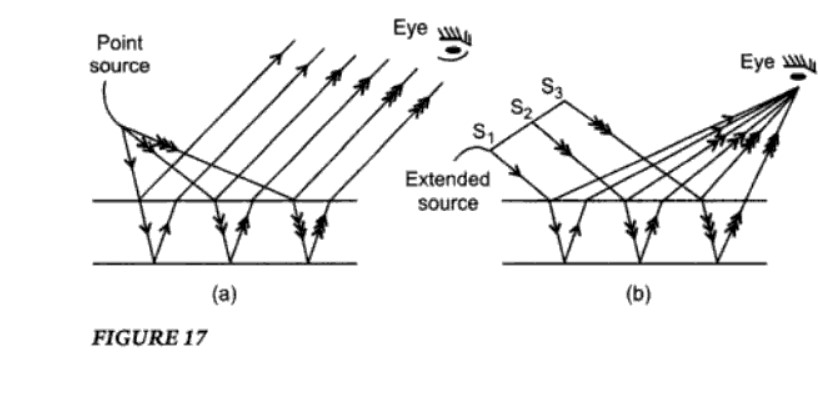
\includegraphics[scale=0.6]{1.jpg}
	\caption{تفاوت منبع نور نقطه ای و منبع نور گسترده در تداخل سنج ها}
	\label{Fig1}
\end{figure}

\noindent
پس استفاده از منبع نور گسترده به این دلیل نیست که فریز ها دیده نمی شوند، بلکه به این دلیل است که میدان دید مشاهده گر محدود است.
\section{ گسترده شدن و جمع شدن نوارهای تداخلی در تداخل سنج مایکلسون با تغییر طول بازوهای تداخل سنج
}
همانطور که از طرح شماتیک این تداخل سنج می توان دید (شکل 
\ref{Fig2}
)
با تغییر فاصله ی بین دو آینه، فریز ها گسترده یا منقبض می شوند. حال اگر آینه ی ۱ را عقب تر ببریم یا طول بازو را زیاد کنیم، پرتو بازتابی از آینه شماره ۱ ، در فاصله دورتری به پرده 
\LTRfootnote{Screen}
 می رسد و این یعنی فریز متناظر دورتر می افتد، پس با افزایش طول بازوها، نوارهای تداخلی دایروی گسترده تر می شود.
\begin{figure}[h]
	\centering
	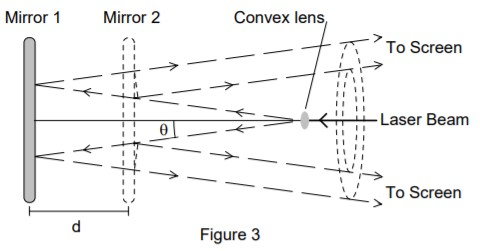
\includegraphics[scale=0.85]{2.jpg}
	\caption{شماتیک تداخل سنج مایکلسون}
	\label{Fig2}
	\end{figure}

\noindent
متناظرا می توان نتیجه گرفت که با کاهش طول بازو ها، نوارهای تداخلی دایروی جمع و جمع تر می شوند
\section{ اندازه گیری ضریب شکست یک گاز در دما و فشار معین با تداخل سنج مایکلسون
}
این هم سوال جالبی است. تصویر زیر را که چینش آزمایش برای اندازه گیری ضریب شکست یک گاز است در نظر بگیرید.
\begin{figure}[h]
	\centering
	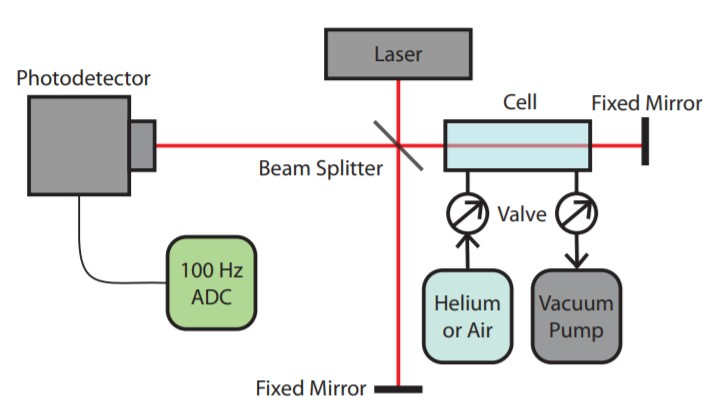
\includegraphics[scale=0.7]{3.jpg}
	\caption{شماتیک تداخل سنج مایکلسون}
	\label{Fig3}
\end{figure}

\noindent
در تصویر
\ref{Fig3}
، یک تداخل سنج مایکلسون می بینیم با این تفاوت که هر دو آینه آن ثابت هستند و در یکی از بازوها، یک سلول به طول 
$d$ قرار دارد که
می تواند محتوی گاز باشد. یعنی با کمک پیچ های تنظیم که مشخص شده اند، می توان گاز را وارد یا خارج کرد. همچنین با تنظیم مقدار گازی که درون سلول است و همچنین دمای محیط می توان به فشار و دمای دلخواه گاز برای اندازه گیری ضریب شکست دست یافت.

\noindent
حالا اگر در حالتی که سلول خالی باشد تصویر فریزها را ببینیم و آرام آرام گاز را درون سلول تزریق کنیم تا به فشار مد نظر برسد و تعداد فریزهایی که شیفت پیدا کرده است را پیدا کنیم، با داشتن طول موج اشعه ای که از سلول عبور می کند و با کمک رابطه ی زیر می توانیم به راحتی ضریب شکست را پیدا کنیم:
\[
m\lambda =2d(n-1)
\]
که در آن $n$ ضریب شکست گاز است.










\end{document}ظ